\section{Кислотность по Бренстеду, сопряженные кислоты и основания. Вода как кислота и основание. Автоионизация воды, ион гидроксония. pH растворов. Расчет pH растворов слабых кислот и оснований.}

\subsection{Кислотность по Бренстеду}

По Бренстеду \textbf{кислоты} --- соединения, которые способны принимать протон, т.е.:

\begin{equation}
	\ce{A H + B <-> A- + H B+}
\end{equation}

Здесь \ce{A H} и \ce{HB+} --- кислоты, \ce{A-} и \ce{B} --- основания. При этом \ce{A H} и \ce{A-}, а также \ce{H B+} и \ce{B} называются \textbf{сопряженными кислотно-основными парами}.


По Бренстеду, вода (\ce{H2O}) может выступать как в роли основания, так и в роли кислоты. Например, при растворении серной кислоты в воде последняя выполняет роль основания:

\begin{equation}
	\ce{H2SO4 + H2O -> H3O+ + HSO4-}
\end{equation}

С переходом протона взаимодействующие соединения поменялись ролями - серная кислота превратилась в сопряженное основание, а вода (основание) - в сопряженную кислоту \ce{H3O+}.

Если же в воде растворяется основание, то она выполняет роль кислоты и в общем случае происходит следующее:

\begin{equation}
	\ce{B + H2O -> HB+ + OH-}
\end{equation}

В силу указанных свойств волна способна к самоионизации:

\begin{equation}
	\ce{H2O + H2O <-> H3O+ + OH-}
\end{equation}

Указанный ион \ce{H3O+} называется \textbf{ионом гидроксония}. Рассмотрим константу равновесия для ионизации воды:

\begin{equation}
	K = \frac{a_{\ce{H3O+}} \cdot a_{\ce{OH^-}}}{a^2_{\ce{H2O}}} = \frac{a_{\ce{H+}} \cdot a_{\ce{OH-}}}{a_{\ce{H2O}}}
\end{equation}

Здесь $a$ --- активность (эффективная (кажущаяся) концентрация компонентов с учётом различных взаимодействий между ними в растворе, то есть с учётом отклонения поведения системы от модели идеального раствора).

Дальнейшее не факт что стоит говорить: \textit{Последнее равенство достигается в предположении, что сумма химических потенциалов \ce{H+} и \ce{H3O+} формально равна удвоенному химическому потенциалу \ce{H2O} в тех же условиях.}

Активность воды примерно равна 1, поскольку большинство кислотно-основных растворов обычно очень разбавлены. Кроме того, в разбавленных растворах активность частиц растворенного вещества примерно равна их \textit{молярной} концентрации. Тогда получится, что:

\begin{equation}
	K = K_w = [\ce{H+}][\ce{OH-}]
	\label{eq:16.water_const}
\end{equation}

При 25$^\circ$C величина $K_w$ является важной константой и равна $K_w = 10^{-14}$.

\subsection{pH растворов}

Для определения кислотности растворов вводится величина, характеризующая концентрацию ионов водорода:

\begin{equation}
	\text{pH} = -\lg [\ce{H+}]
\end{equation}

Строго говоря, под логарифмом должна стоять активность, но мы скажем, что она примерно равна молярной концентрации (моль/литр).

pH$<7$ соответствует кислотному раствору, в то время как pH$>7$ --- основному.

Для определения pH раствора используются \textit{индикаторы}, меняющие свой цвет в зависимости от среды (см. рисунок \ref{fig:16.colors}).

\begin{figure}[H]
	\centering
	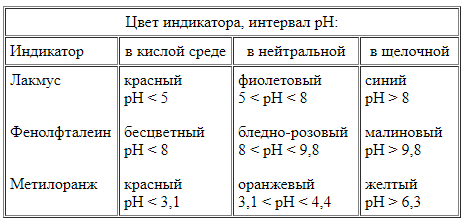
\includegraphics{16.colors}
	\caption{Цвета различных индикаторов в зависимости от pH среды}
	\label{fig:16.colors}
\end{figure}

Для работы с слабыми кислотами и основаниями, которые распадаются на ионы не полностью, а концентрация ионов \ce{H+}, например, в растворе слабой кислоты уже не равна концентрации самой кислоты, используется \textbf{закон разбавления Оствальда} для слабых электролитов (опустим его вывод, сказав лишь, что [не факт, что стоит говорить] \textit{получается он из закона действующих масс}). Согласно ему:

\begin{equation}
	K = \alpha^2 c
\end{equation}

Здесь $K$ --- постоянная диссоциации, $c$ --- концентрация слабого электролита в моль/литр, $alpha$ --- \textbf{степень диссоциации}, т.е. отношение числа продиссоциированных молекул вещества к общему числу молекул.

На основании этого:

\begin{equation}
	\alpha c = \sqrt{\frac{c^2 K}{c}} = \sqrt{K c}
\end{equation}

\underline{Для слабых кислот (вместо $K$ пишем $K_a$):} 

\begin{equation}
	[\ce{H+}] \approx \alpha c \qrq \boxed{\text{pH} = \frac{1}{2} \left(pK_a - \lg c\right)}, \quad \text{где } pK_a = -\lg K_a
\end{equation}

\underline{Для слабых кислот (вместо $K$ пишем $K_b$):} 

\begin{align*}
	[\ce{OH-}] \approx \alpha c \qrq \text{pOH} = \frac{1}{2} \left(pK_b - \lg c\right) \qrq\\
	\qrq \boxed{\text{pH} = 14 - \text{pOH} = 14- \frac{1}{2} \left(pK_b - \lg c\right)}, \quad \text{где } pK_b = -\lg K_b
\end{align*}

Последнее равенство тривиально следует из \ref{eq:16.water_const}.







